\begin{figure}[H]
\centering
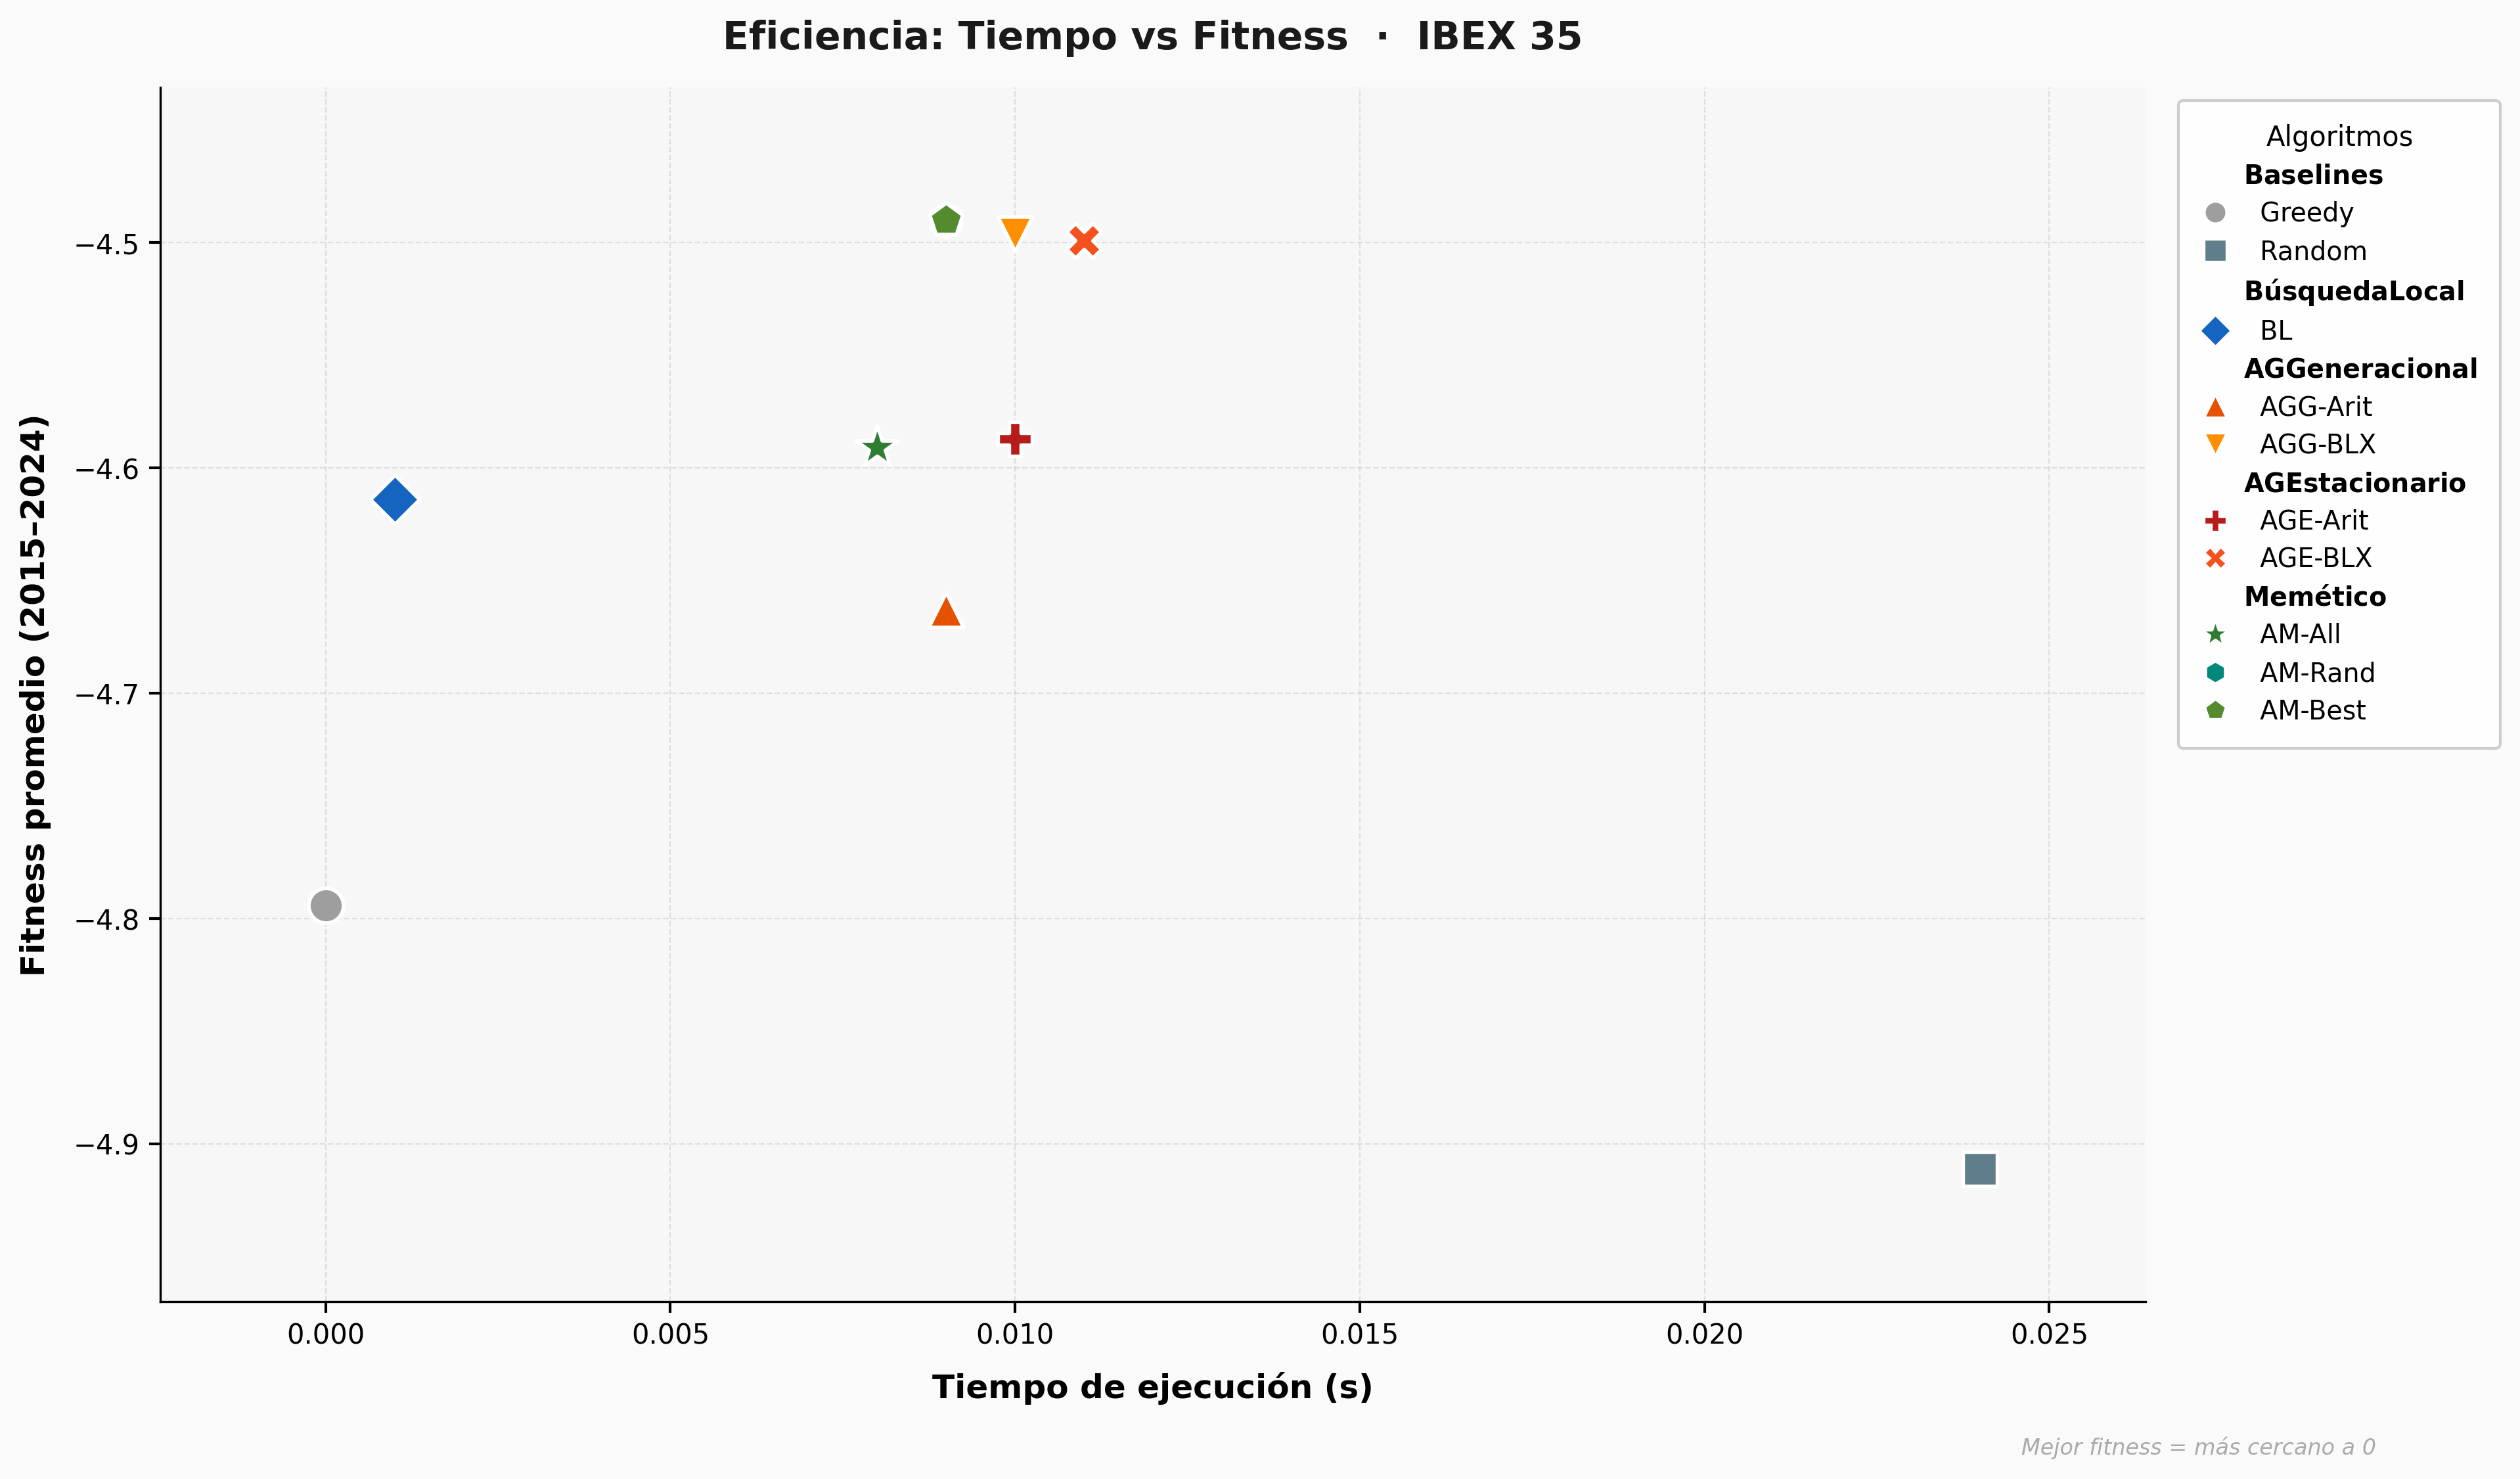
\includegraphics[width=0.90\textwidth]{figuras/eficiencia_IBEX_35.png}
\caption{Análisis de eficiencia: Tiempo de ejecución vs Fitness promedio --- IBEX 35. Cada punto representa el promedio de 50 ejecuciones independientes. \textit{Nota:} Los puntos correspondientes a AM-Rand y AM-Best se solapan debido a su práctica identidad en tiempo y fitness.}
\label{fig:eficiencia-ibex}
\end{figure}

En el IBEX~35, el tiempo de ejecución es negligible para todos los algoritmos (máximo 0.024~s), lo que refleja la naturaleza de baja dimensionalidad del problema (35 activos). Greedy es instantáneo pero ofrece un fitness mediocre por su falta de exploración global. Random invierte ligeramente más tiempo sin mejorar significativamente la calidad, demostrando la ineficacia de la búsqueda sin estructura en espacios incluso pequeños. Los algoritmos poblacionales (AG y AM) convergen en un rango de fitness superior en torno a un 2--4\,\% mejor que Random, con un coste computacional prácticamente imperceptible. AM-Rand y AM-Best logran la mejor relación costo-beneficio en este mercado: en una fracción de milisegundo alcanzan soluciones de calidad comparable a AGG-BLX.

\begin{figure}[H]
\centering
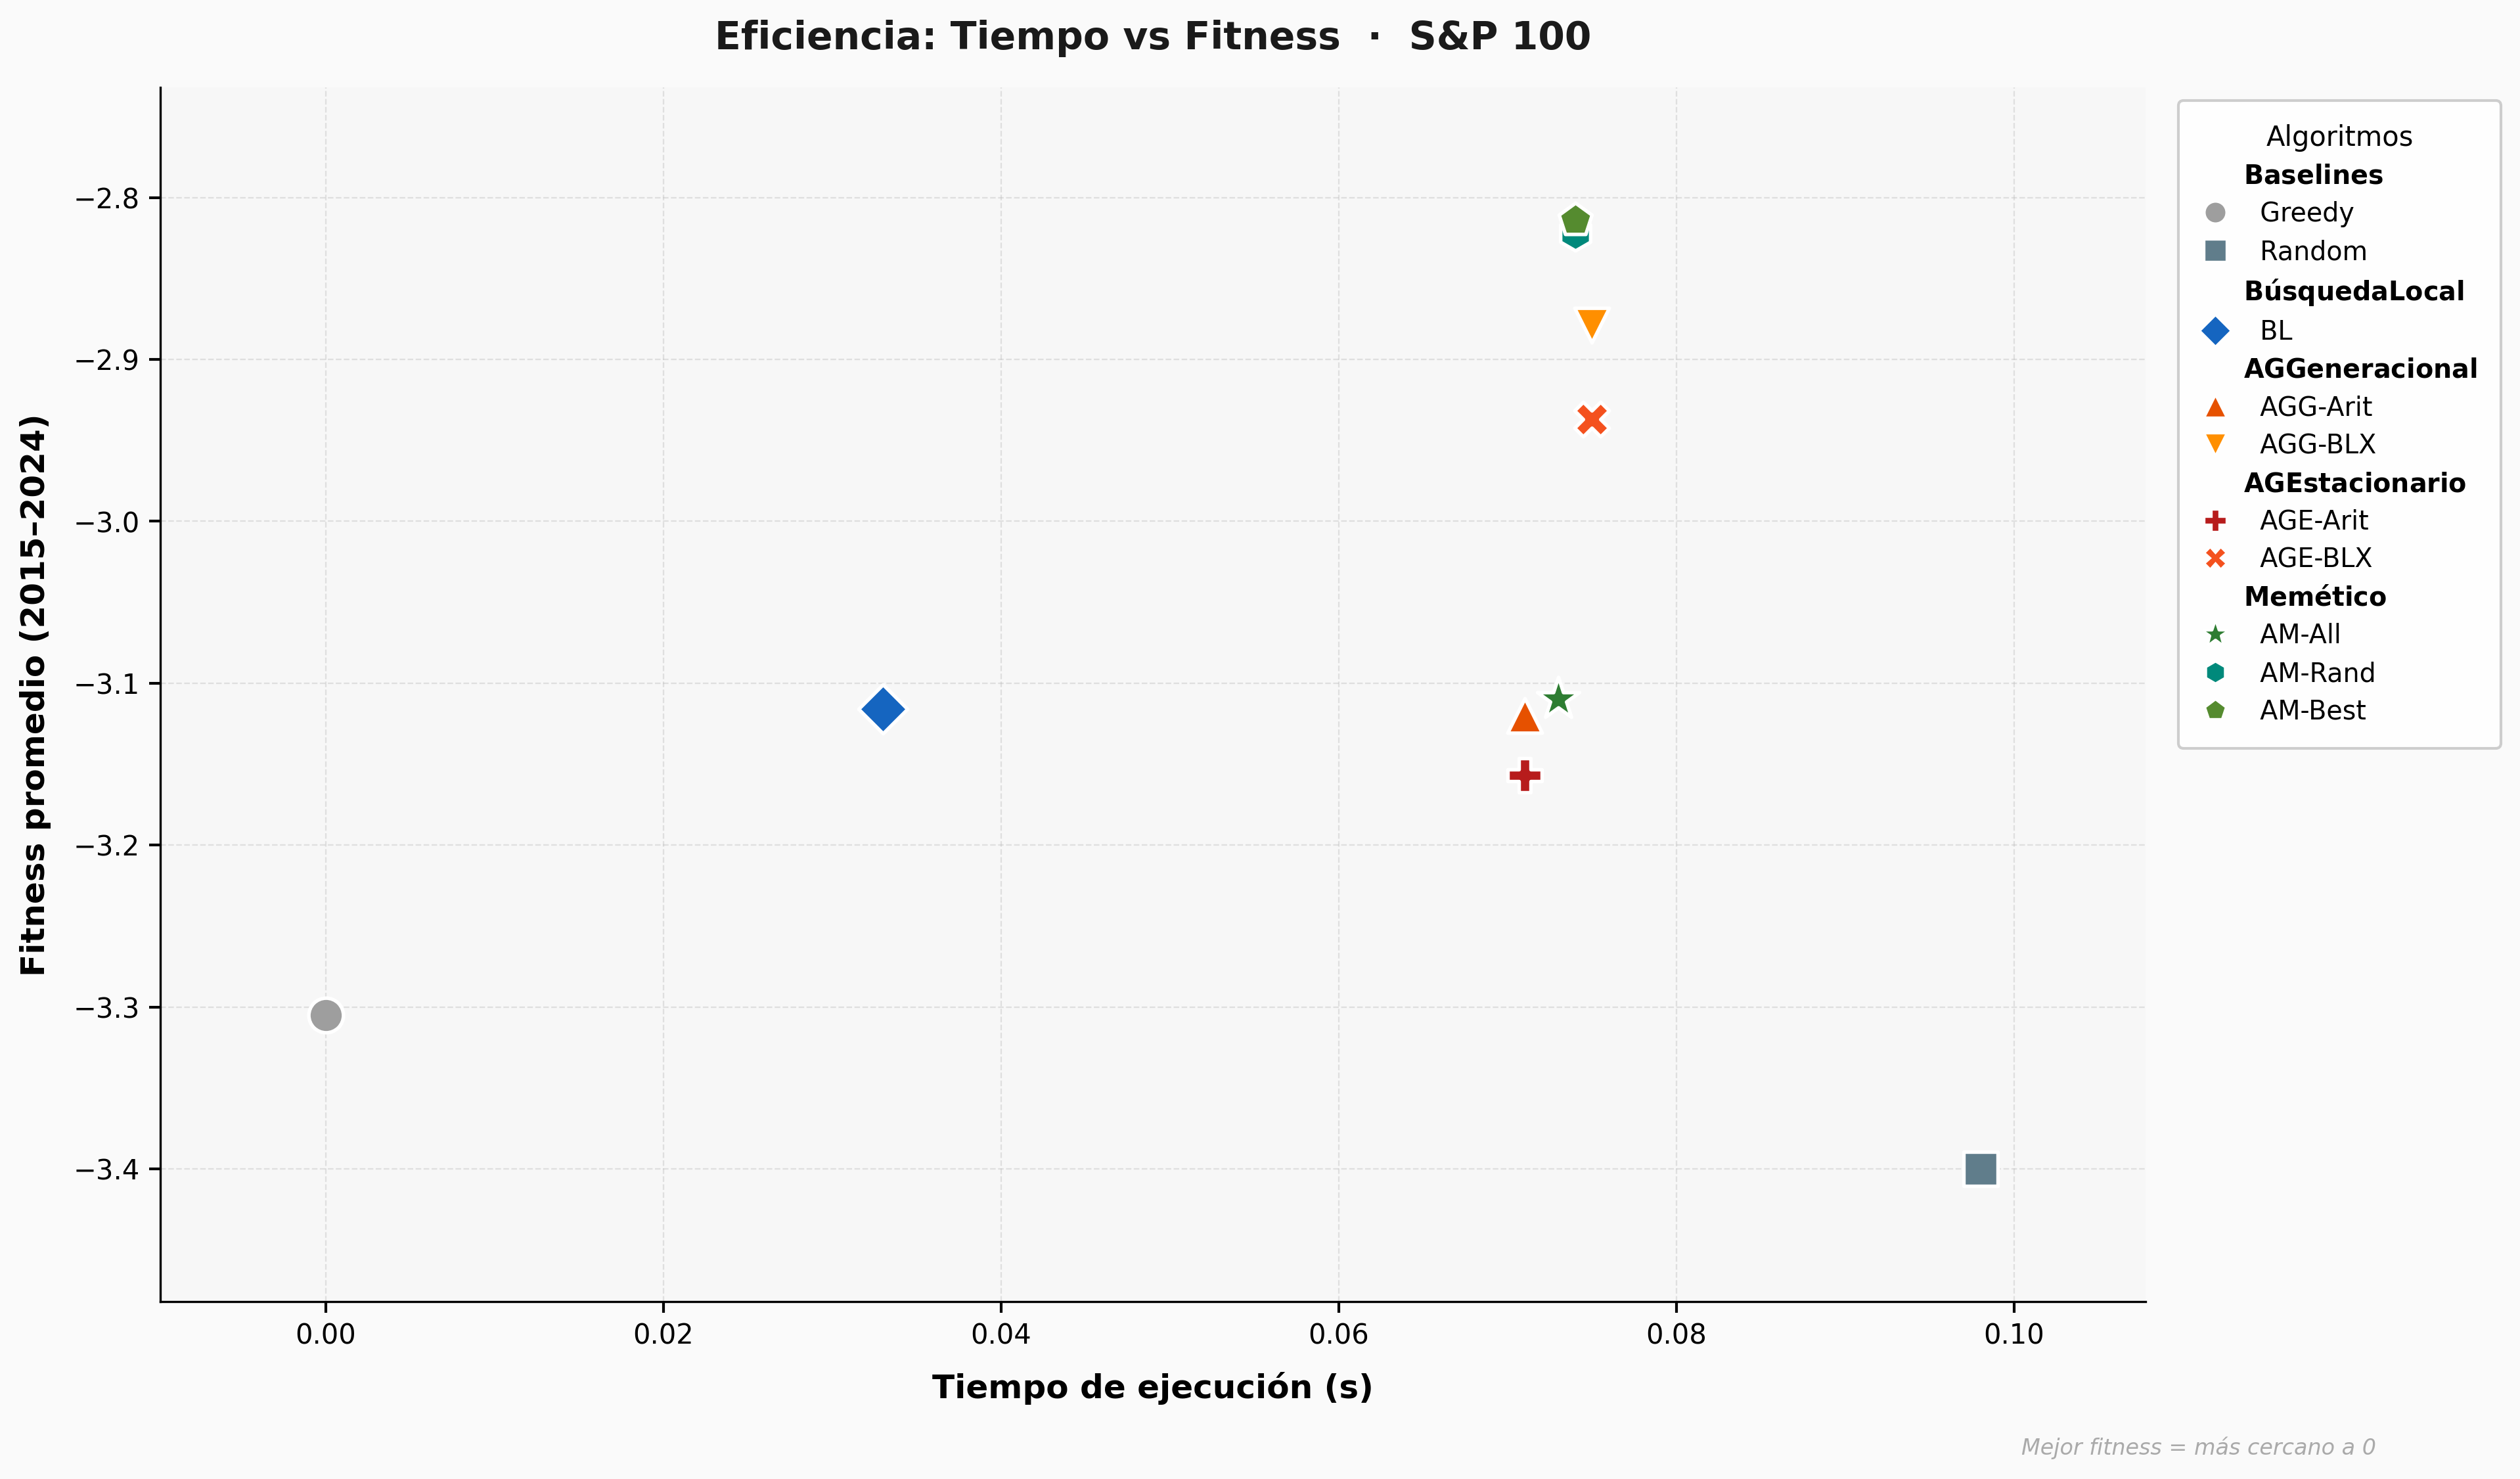
\includegraphics[width=0.90\textwidth]{figuras/eficiencia_SP_100.png}
\caption{Análisis de eficiencia: Tiempo de ejecución vs Fitness promedio --- S\&P 100. Cada punto representa el promedio de 50 ejecuciones independientes. \textit{Nota:} Múltiples algoritmos meméticos y genéticos presentan tiempos muy similares (0.071--0.075~s) formando un cluster denso.}
\label{fig:eficiencia-sp100}
\end{figure}

El S\&P~100 exhibe un patrón más estratificado. Greedy sigue siendo prácticamente instantáneo pero inferior en fitness. Random consume entre 4 y 5 veces más tiempo que Greedy, revelando la sobrecarga de exploración aleatoria, y su calidad apenas mejora. BL requiere más tiempo que Random (0.033~s frente a 0.098~s) pero se sitúa a mitad de camino entre Random y los poblacionales en términos de fitness. Los algoritmos genéticos puros forman un cluster donde AGG-BLX destaca con aproximadamente un 5--7\,\% de mejora sobre Random, mientras que las variantes aritméticas quedan ligeramente por debajo. AM-Rand y AM-Best se sitúan en la frontera de Pareto: requieren un tiempo muy similar a AGG-BLX pero consiguen un fitness entre un 2\,\% y un 4\,\% superior, consolidando su posición como la mejor opción en relación costo-beneficio.

\begin{figure}[H]
\centering
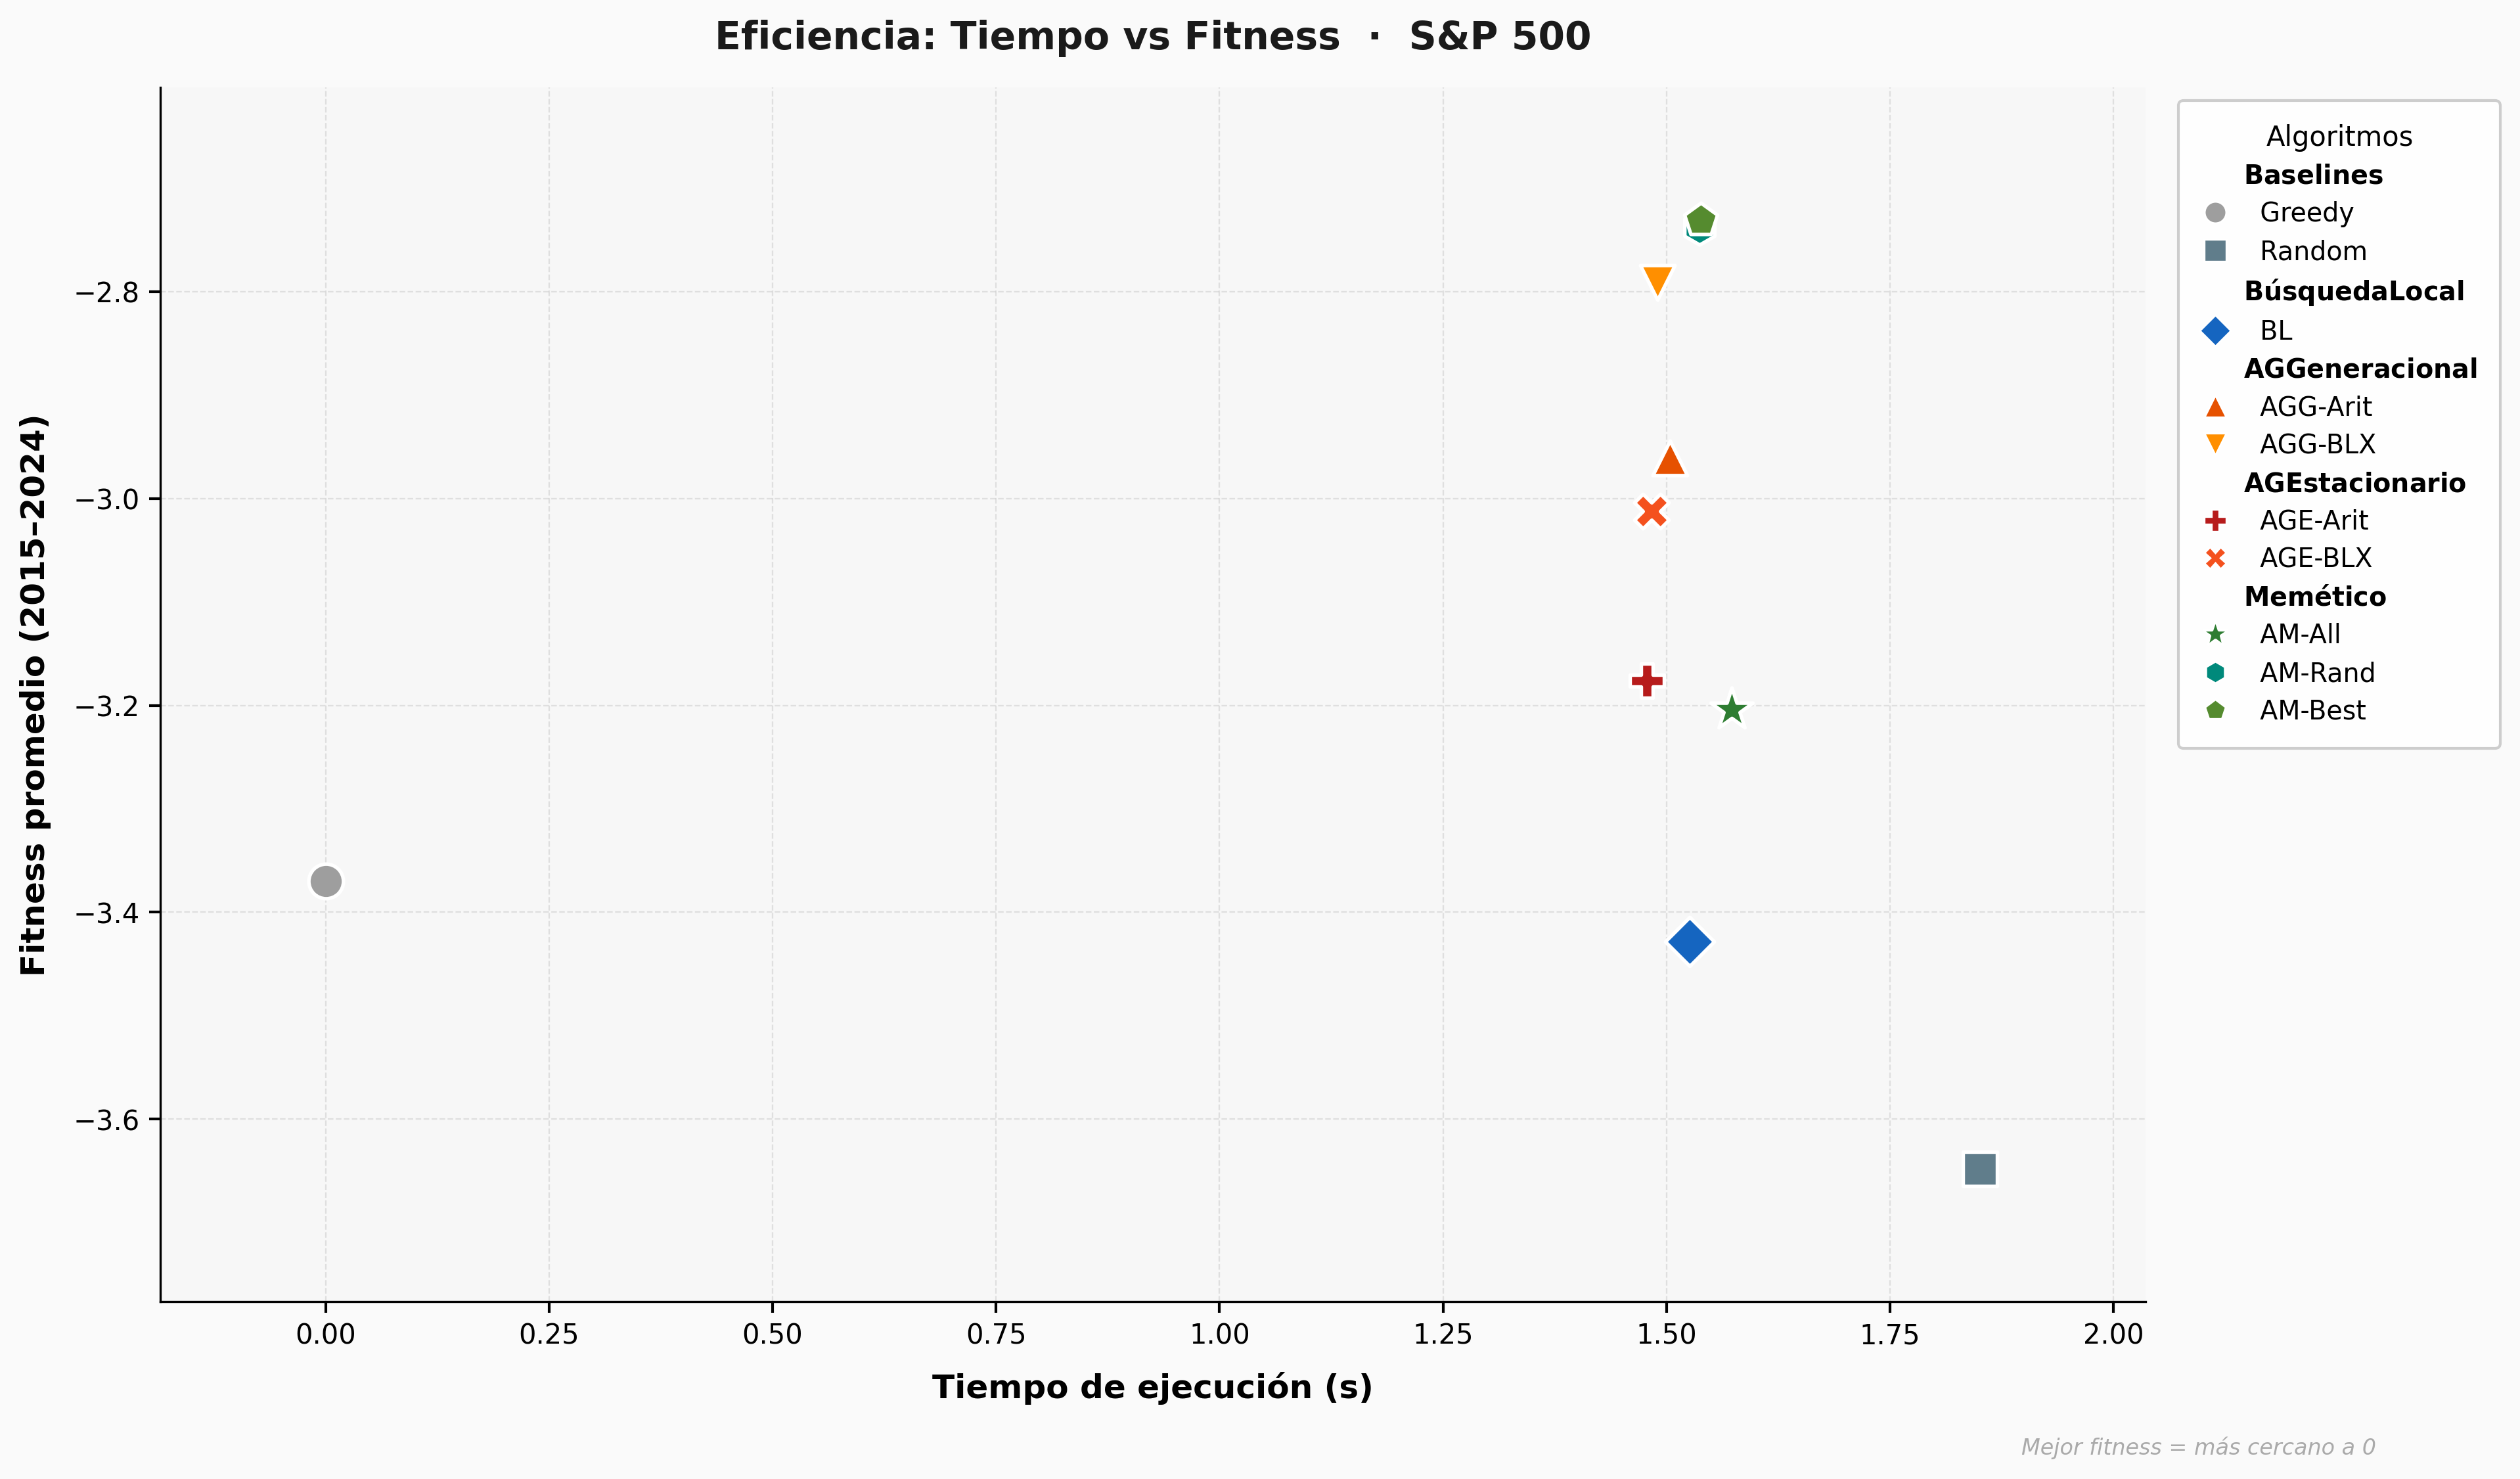
\includegraphics[width=0.90\textwidth]{figuras/eficiencia_SP_500.png}
\caption{Análisis de eficiencia: Tiempo de ejecución vs Fitness promedio --- S\&P 500. Cada punto representa el promedio de 50 ejecuciones independientes. \textit{Nota:} Los algoritmos poblacionales (genéticos y meméticos) forman un cluster muy denso en torno a 1.48--1.54~s de tiempo.}
\label{fig:eficiencia-sp500}
\end{figure}

El S\&P~500, con su dimensión de 500 activos, amplifica las diferencias y revela las limitaciones de cada enfoque. Greedy sigue siendo instantáneo pero su calidad es ahora dramáticamente inferior (aproximadamente un 20\,\% peor que los mejores poblacionales). Random consume un tiempo colosal (1.85~s) ---comparable al de los algoritmos poblacionales--- pero no logra ventaja de calidad: permanece en una zona inferior a todos los poblacionales, demostrando el fracaso de la exploración sin estructura en espacios de alta dimensión. BL requiere 1.53~s, un tiempo similar a Random, pero logra mejorar la calidad en aproximadamente un 8--12\,\% respecto a Random, mostrando el poder de la explotación local una vez que se tiene una buena solución inicial. Los algoritmos genéticos puros invierten tiempo comparable a BL (1.48--1.51~s) pero alcanzan una calidad sustancialmente superior, entre un 15\,\% y un 25\,\% mejor que Random, demostrando que la evolución poblacional supera ampliamente a la búsqueda local aislada en espacios grandes. AM-All constituye un outlier negativo: consume tiempo (1.57~s) pero logra un fitness inferior al de AGG-BLX, corroborando que la aplicación indiscriminada de BL es contraproducente. AM-Rand y AM-Best emergen como los claros ganadores: requieren tiempo apenas superior a AGG-BLX (1.54~s) pero alcanzan una calidad entre un 2\,\% y un 3\,\% superior, representando el equilibrio óptimo entre velocidad y precisión en el problema de cartera de alta dimensión.
